\documentclass[11pt, twocolumn]{article}
\usepackage[utf8]{inputenc}
\usepackage[english]{babel}
\usepackage{quoting}
\usepackage{csquotes}
\usepackage{enumitem}
\usepackage{natbib}
\usepackage{xparse}
\usepackage{url} 
\usepackage[breaklinks=true]{hyperref}
\usepackage{color}
\usepackage{graphicx}
\usepackage[margin=1in]{geometry}
\usepackage[ruled,vlined]{algorithm2e}


\usepackage[backend=biber, sorting=none]{biblatex}
\addbibresource{references.bib}

% \usepackage{geometry}
%  \geometry{
%  a4paper,
%  total={170mm,257mm},
%  left=30mm,
%  right=30mm,
%  top=25mm,
%  }

% fix boldness bug
\begin{document}
%% Article's information:
% \title{Robots and Slavery - Is that a thing? }
\title{A comparative study on different Models for Community Detection.}
%% Author's information:
% \author{Olusanmi Hundogan\\M.Sc. Artificial Intelligence\\Utrecht University\\o.a.hundogan@students.uu.nl}

\maketitle
\begin{abstract} 
This paper deals with community detection and answers the question about the role of models and quality functions within community detection. For that purpose compares the performance of different quality functions while keeping a fixed partitioning heuristic. The paper also introduces a novel approach to community detection by emploing node embeddings learned by the GloVe method. The results show that the quality function does play an important role in the performance, but requires algorithmic procedures to mitigate idiosyncratic short-comings of the model. The paper also shows that similarity-based methods can yield promising results if coupled with Deep Learning techniques. 
\end{abstract}
%%

%%%%%%%%%%%%%%%%%%%%%%%% Main text: %%%%%%%%%%%%%%%%%%%%%%%%
\section{Introduction}
Finding and understanding communities is one of the most prominent tasks in network science. Various applications range from finding communities in social networks, searching the web or predicting the spreading behaviour of a pandemic. There are many ways to define a community, but a modern perspective describes communities as a set of densely connected vertices in which the intra-community connections probability is substantially higher than the extra-community connections.\cite{fortunato_CommunityDetectionNetworks_2016} There has been a multitude of algorithms developed in recent years and \citeauthor{lancichinetti_CommunityDetectionAlgorithms_2009} showed that InfoMap and the Louvain algorithm are among the most successful ones.\cite{lancichinetti_CommunityDetectionAlgorithms_2009} Both algorithms are optimization based with different quality functions as objective. More recently similarity-based methods have seen a resurgence due to the increased interest in deep learning and graph embeddings in recent years.\cite{liu_DeepLearningCommunity_2020} Another trait of both, Louvain and Infomap, is their algorithmic similarity of partitioning the graph.\cite{rosvall_MapEquation_2009} This ultimately begs the question how important the model is and which of these models show cases the best performance in terms of finding relevant communities? For this purpose, the paper will keep a Louvain-inspired core algorithm unchanged and compare different quality functions as objectives.\cite{blondel_FastUnfoldingCommunities_2008} Additionally, this paper will introduce a novel algorithm for community detection to incorporate a modern similarity based quality function into the analysis. 
The paper is structured as follows: After reviewing the related work in Section \autoref{sec:rel_work}, Section \autoref{sec:experiment} will begin with the experimental setup, which includes a description of the Louvain algorthm, the benchmark graphs that will be use and the comparison metric. Thereafter, Section \autoref{sec:models}, will explain the various models that will be used in the analysis. It will additionally introduce briefly a novel approach to detect communities based on graph embeddings and Louvain-Core. Then, Section \autoref{sec:results} will present the results of the analysis. This will be followed by a general interepretation of the result in Section \autoref{sec:discussion} and finally, Section \autoref{sec:summary} will summarize the paper.

\section{Related work}
\label{sec:rel_work}
As mentioned earlier, several methods have been introduced for the purpose of detecting communities.\cite{fortunato_CommunityDetectionGraphs_2010} These methods use various properties of graphs that can range from structural, dynamic, spectral to stochastic approaches. Some of the examples would be graph partitioning, k-clustering or spectral clustering. Fortunato provides two exhaustive studies in \citeyear{fortunato_CommunityDetectionGraphs_2010} and \citeyear{fortunato_CommunityDetectionNetworks_2016} on various aspects of community detection including many different techniques used within the scientific community. The formalization of Modularity as a quality measure by \citeauthor{newman_FindingEvaluatingCommunity_2004} has led to more recent optimization-based algorithms that have proven to be fast, efficient and robust approximations of the true partition.\citeyear{fortunato_CommunityDetectionGraphs_2010} An earlier example would be the method by \citeauthor{clauset_FindingCommunityStructure_2004}, but more popular methods are the Louvain algorithm and InfoMap. All of the methods share the heuristic idea to iterate through network nodes and greedily assign communities based on adjacent partitions which maximize a particular quality function. However, Louvain and InfoMap additionally incorporate aggregation phases to speed up the partitioning process. These ideas will also be used in the Louvain-Core algorithm, present in this paper. With this paper's novel approach in mind, it is important to note that similarity based approaches have largely failed to capture the same popularity as Louvain or InfoMap. Mainly, because it is hard to define an appropriate representation of a node which captures all the necessary structural information to capture communities. Additionally, graphs in community detection are often sparse and representations high-dimensional which renders data-driven models ineffective.\cite{cai_ComprehensiveSurveyGraph_2018} However, another scientific, yet largely unrelated, community made significant progress with similar challenges due to the emergence of Deep Learning techniques. The invention of the Skip-Gram Model by \citeauthor{mikolov_DistributedRepresentationsWords_2013} renewed interest into the field of computational word semantics.\cite{mikolov_DistributedRepresentationsWords_2013} Here, the model uses neural networks to learn low-dimensional word representations by maximizing co-occurrence probabilities. Several similar models followed: Variants like FastText, WordRank or GloVe have been applied in numerous contexts.\cite{alvarez_ReviewWordEmbedding_} These ideas can be applied to graphs because random walk node sequences resemble word sequences. DeepWalk and node2vec are popular examples among many. For more examples see \citeauthor{cai_ComprehensiveSurveyGraph_2018}'s review.\cite{cai_ComprehensiveSurveyGraph_2018} Approaches that apply node embeddings to community detection are still rare but typically use the Skip-Gram approach or a slight modificaion. \citeauthor{rozemberczki_GEMSECGraphEmbedding_2019}'s GEMSEC model is a recent example.\cite{rozemberczki_GEMSECGraphEmbedding_2019} However, the novelty of this papers' algorithm lies in the use of GloVe to train node embeddings and combine it with the Louvain Core algorithm.\cite{pennington_GloveGlobalVectors_2014} GloVe is particularly interesting, because it harnesses ideas from matrix factorization methods like LSA and local context window approaches like Skip-Gram.  

\section{Experimental setup}
\label{sec:experiment}
The analysis is done by comparing the performances of various models on undirected graphs. The experiment is written in Python and can be executed as python script. The benchmarks are publicly available and the comparison metric was implemented by the author. However, there are also publicly available implementations of the comparison metric. More details on how to download and execute the experiment are in the attachment section or on Github where the code for this paper resides. This is also the location for more recent explanations on the code usage.

\subsection{Preliminaries}
As a prerequisite, it is necessary to establish some of the notations used in this paper. First, $G(V,E)$, $C$ and $P$ refer to a Graph, a community and a partition (which is a set of communities), respectively. $|V|= n$ are the number of vertices and $|E|=m$ is the number of edges. $p_{in}$ is the probability that a randomly chosen vertex within a community connects to another vertex from that same community. Likewise, $p_{ex}$ refers to the probability to connect to a vertex outside of the community. $A$ denotes the adjacency matrix of a graph and subscripts $i$ and $j$ its individual entries.

\subsection{LFR - Benchmark}
In order to compare these models fairly, the benchmark on which they apply must be stable, fast and well-researched. This automatically excludes many real-world network data sets. Hence, the analysis will resort to artificially created graphs as benchmark which sufficiently approximate the behaviour of real world networks. A popular benchmark for community detection was proposed by \citeauthor{girvan_CommunityStructureSocial_2002}, with a number of planted equally sized partitions and a fixed average node degree. It is based on the popular idea that vertices have a higher connection probability to vertices inside their respective community than outside ($p_{in} > p_{ex}$). However, most real-world networks do not display this behaviour, as the degree distribution of many real-world networks are heterogenous.\cite{lancichinetti_CommunityDetectionAlgorithms_2009} Hence, this paper will use the LFR model as a benchmark, because its community sizes and degree distributions follow the power-law distribution. $\tau_1$ and $\tau_2$ act as exponents for the power-law distributed degrees and community sizes, respectively. Further, the model introduces a mixing parameter $\mu$ which acts as an upper bound for the ratio between the external degree of a graph and its total degree. $\mu$ only depends on the network size and the size of the largest community and ensures the model remains well defined. Noteworthy, is the fact that communities are, are in principle detectable until $\mu<0.75$. Meaning, every model will break down after that threshold. For more details on the specific benchmark and its characteristics, see the original paper by \citeauthor{lancichinetti_CommunityDetectionAlgorithms_2009}. For this comparative analysis, both, $\tau_1$ and $\tau_2$, will remain fixed at -2 and -1, while $\mu$ will increase linearly from 0.1 to 0.8. This paper will present, two curves for each model which align with the chosen node size 250. The reported values will be averaged over ten runs per configuration. The overall experimental setup is largely inspired by \citeauthor{lancichinetti_CommunityDetectionAlgorithms_2009}'s experiment but smaller in scale, as the Louvain-core algorithm and the map-equation model are implemented in python which is significantly slower than typical implementations in C/C++.      


\subsection{Normalized Mutual Information} 
In literature, many metrics have been proposed to compare two partitions with one another. Many of them are rooted in clustering algorithm literature, due to similarities between community detection and clustering. In both the cases the metrics have to represent how closely a partition $P$ resembles the true partition. However, only a few of them are popular due to some of the idiosyncrasies in community detection. Metrics such as the Jaccard or Rand index are not normalized, while the \emph{fraction of correctly identified nodes} is not very well defined for case that are frequently encountered within community detection. For further information see \citeauthor{fortunato_CommunityDetectionNetworks_2016}. This paper will use the Normalized Mutual Information (NMI) score, due to its reliability. It is rooted in information theory and the idea is to measure how much information one partition yields about another. Mutual information can be measured in terms of the joint entropy of two random variables X and Y which represent the cluster assignments of the predicted and true partition, respectively. However, this metric is not normalized which is why we further divide by the sum of X and Y's entropies (H(X) and H(Y)). 

\begin{equation}
I(X,Y) = \sum_x\sum_y P(x,y) log\frac{P(x,y)}{P(x)P(y)}
\end{equation}
\begin{equation}
I_{norm}(P_{pred},P_{true}) = \frac{2I(X,Y)}{H(X) + H(Y)}
\end{equation}

\subsection{Louvain Algorithm (Core)}
As mentioned in the introduction, both -- the model and the optimization algorithm -- are separable and can be compared independently. As this paper is going to focus on the model, the optimization algorithm will remain fixed. This paper will use the Louvain-Algorithm by \cite{blondel_FastUnfoldingCommunities_2008}. The Louvain-Algorithm is a heuristic method and in essence a more efficient variant of the algorithm by \citeauthor{clauset_FindingCommunityStructure_2004}. The core of the algorithm can be divided in two phases:\cite{waltman_SmartLocalMoving_2013} First, all vertices are traversed in a random sequential order. For each vertex a quality function will evaluate whether moving the node to a community of an adjacent vertex yields an increase of the quality function's output. If that is the case, the node will be moved to that community, otherwise it remains in his community. This procedure will be repeated, until no movement results in any further increase. The paper will refer to this as \emph{local movement phase}. This initiates the second phase, the \emph{reduction phase}, in which the current communities are aggregated into a reduced graph. The nodes of this graph will contain a self-edges, whose weight will reflect the total amount of nodes aggregated in that respective community. Edges to other reduced vertices are taken from the total amount of edges that connected the communities in the original graph. Both phases will repeat until no further changes are applied and the maximal output is attained. The iterative application of both phases will be coined as core algorithm, as it is indifferent to the quality function and therefore the underlying model. The next section will discuss several quality functions that will be evaluated in the comparative analysis. However, it is worth mentioning that the algorithm \emph{maximises} the output of the quality function. Therefore, modifications are required if the model expects the \emph{minimization} of the quality function. But these modifications are trivial, because any minimization problem can be turned into a maximization problem by multiplying with -1. 

\section{Models}
\label{sec:models}
The paper will compare the NMI results of several models. For this purpose, a model refers to the underlying principle that governs the evaluation of the "fitness" of a particular partition. Core models are founded in modularity, information science and node similarity. The core algorithm was implemented by the author to ensure that it remains fixed for all models. Most of the quality functions in use are publicly available. However, the map equation model was implemented from scratch as the only publicly available version is written as part of InfoMap and is hard to use independently.


\subsection{Modularity}
Modularity is probably the most popular quality function within the community detection literature.\cite{fortunato_CommunityDetectionGraphs_2010} It is able to measure the strength of separability of partitions and commonly used for optimization-based techniques. The notion is that a graph with a particular community structure is noticeably different from a random graph which preserves some of the original partitioned graph's features but destroys the community structure. Modularity is defined by \autoref{eq:modularity}.

\begin{equation}
    \label{eq:modularity}
    Q = \frac{1}{2m}\sum_{i,j}(A_{ij}-N_{ij})\delta(C_i,C_j)
\end{equation}

Here, $N$ represents the randomized copy of the graph. It is often called null model and can be defined in various ways, but the most common representation is $N_{ij} = \frac{k_ik_j}{2m}$. $\delta(C_i, C_j)$ is the kronecker-delta of both communities, meaning only vertices that belong to the same community contribute to the averaged distance. The model works well for a number of network, but it is widely known that the original definition suffers from resolution issues. This becomes an issue for networks with sub-community structures or small communities. \citeauthor{lancichinetti_CommunityDetectionAlgorithms_2009} shows how greedy modularisation models like the one from \citeauthor{clauset_FindingCommunityStructure_2004} broke down early when the mixing parameter increased.\cite{lancichinetti_CommunityDetectionAlgorithms_2009} However, the hierarchical nature of the Louvain-Core algorithm appears to mitigate resolution issues. 
\subsection{Map-Equation}
The next model is based on flow dynamics of networks and was proposed by \citeauthor{rosvall_MapEquation_2009}.\cite{rosvall_MapEquation_2009} The core intuition is that a random walker on a network will remain "trapped" in communities before exiting and changing to another. By encoding the individual nodes and transitions to other communities we can encode the path of a random walker and compute the average codelength. This, in turn, corresponds with the entropy of encoding the node-visit and community-transition probabilities. Lower entropy corresponds with the more efficient encoding of the random walk. Finding the lowest entropy amounts to finding the best partition, which leads to the optimization target. For more information on the underlying intuition see \citeauthor{bohlin_CommunityDetectionVisualization_2014}. The Map-Equation, computes the average code-length $L$ of a partition $P$ and needs to be minimized:

\begin{equation}
    \label{eq:mapequation}
    L(P) = p_{ex} H(Q) + \sum_{i=1}^m p_{in}^iH(P^i)
\end{equation}

In equation \autoref{eq:mapequation}, L represents the function to compute the average code length which is a weighted sum of the transition entropies $H(Q)$ and the community entropies $H(\rho^i)$ for every community $i$. $p_{ex}$ and $p_{in}$ are the probabilities of transitioning and remaining in each module. These probabilities can be estimated by simulating a random walk on a graph. However, it is more efficient to use the power-iteration method on the transition-matrix to obtain the normalized eigenvector. The power-iteration methods is an iterative approach to extract the first eigenvector of a nonnegative matrix. The transition-matrix is a matrix whose elements correspond with transition probabilities. The normalized eigenvector represents the stationary distribution of the matrix. Mainly, the probability distribution to visit any of the nodes in the graph. For undirected networks it is even possible to estimate the probabilities by computing the relative weights of each node. The relative weight is the degree of a node divided by twice the number of edges.            

\subsection{Baselines}
In order to evaluate the importance of a model in general, it is reasonable to include baselines. Coverage is a fairly simple metric. Hence, it will help to distinguish between simple optimization metrics and more sophisticated ones. It describes the ratio between the edges inside the community and the total amount of edges.\cite{fortunato_CommunityDetectionGraphs_2010} This quality function conveys the notion that there are significantly more intra-community edges than inter-community edges. Hence, the best partition is the one which maximizes the coverage. The formula strongly resembles modularity. In, fact modularity can be seen as difference between the partition coverage and the expected coverage of the null model. Hence, it is expected, that this model will perform worse than modularity based approaches, as modularity takes idiosyncracies of the graph into account.

That following algorithms will not utilize any quality function for community detection. For this purpose, the paper will include the performances of a simple label propagation algorithm. Label propagation strongly resembles the local movement of the Louvain algorithm. But uses majority votes of neighbors to apply communities. The decision criteria is simplistic and purely heuristic. Hence, it is suitable as a baseline model, because it does not use any quality function. It was proposed by \cite{raghavan_LinearTimeAlgorithm_2007} and its speed is close to linear time. It works reasonably well for low mixing parameters but tends to favor large communities. This is the reason why it collapses to one community for higher mixing parameters. 

Aside from the reference implementation, the paper will include a Louvain-Core inspired variant. With this, the algorithm will be closer to the other algorithms. However, in order to prevent the partition collapse the first phase will only iterate one time through the nodes. This is in contrast to Louvain-Core, as those local movements reiterate until no changes apply anymore. To the authors knowledge, this is also a novel method which has not been explored so far. Another base line to briefly mention is the random propagation model. It will work wit Louvain-Core, but assign communities of neighbors randomly.

\subsection{Similarity Maximization}
The last model is a novel implementation and combines several key ideas from the natural language processing and community detection literature. This section will only briefly convey the intuition, but the details will be found on GitHub and the attachment section. The algorithm uses Louvain-Core for partitioning. However, the quality function is based on node similarities. The key idea is that nodes will have the lowest distance to their true but latent community centroid. Hence, the best partition minimizes the sum of the centroid distances for each community. This idea is very reminiscent of k-clustering algorithms. However, the strict application is counter-productive for Louvain-Core which starts with each node in its own partition. Hence, the initial sum of the average centroid distances is zero, because each node is maximally close to itself. Therefore, this approach maximizes the "gain" of moving a node from one community to another. The giving community will most probably reduce its average distance to the centroid, while the receiving community will most likely see an increase in its average centroid distance (ACD). Meaning the "gain" can be interpreted as the difference between ACD reduction minus the ACD increase. The ACD increase, however, can also be interpreted as a "gain" if the inclusion of a node reduces the ACD instead of increasing it. This case can be reinforced by maximizing the product of the ACD giver gain and receiver gain. With this objective, the model has every incentive to reduce the amount of partitions in the initial Louvain-Core case, but eventually tries to reduce the partition to large communities. Hence, every ACD gain-product is additionally normalized by the number of nodes in the receiving partition.
\begin{equation}
    ACD(C)= \frac{1}{|C|} \sum^{|C|}dist(C_i, \overline{C})
\end{equation}
% \begin{equation}
%     \Delta ACD(C)= ACD(C)-ACD(C')
% \end{equation}
\begin{equation}
    Gain = \frac{\Delta ACD(R)*\Delta ACD(G)}{|R|}
\end{equation}

$C$ is a set of node representations which capture distances between nodes well. Likewise $C'$ is the same set but modified. That results in a change of the ACD which is the average distance to the centroid $\overline{C}$ of that set. The Gain is the product of the receiving set $R$ and giving set $G$ divided by the set size $|R|$. 

Now, the question remains how to represent the nodes while maintaining their structural information. For this purpose, the algorithm initialises node-embeddings by using GloVe. This model combines global matrix factorization and local context window techniques to learn node representations. It maximizes a co-occurrence matrix and uses the trained parameters as node representation. The co-occurrence matrix can be obtained by counting the co-occurrences of nodes in a random walk. Simply put, a node X co-occurs with another node Y if it appears within a "window" of random walk steps in the past and future of that node Y. More details and the math can be found in the original paper by \citeauthor{pennington_GloveGlobalVectors_2014}. This paper uses the L2-distance function to compute distances between the node embeddings and the centroid is calculated by averaging the node embeddings. For the reduction step in Louvain-Core, the reduced clusters will use their respective centroids as node embedding for the next iteration. A more elaborate description on hyper parameters and the implementation details of the model can be found in the attachment section. 


% TODO: Implementation detail -> The difference must be chosen in such a way that it reflects gain. Meaning different things for R and G.
% TODO: Implementation detail -> Explain that C is set of vectors and distance is L2
% TODO: Random walk sampling 

\section{Results}
\label{sec:results}
As mentioned beforehand each algorithm was tested 10 times on an LFR graph with increasing mixing parameter $\mu$. Each graphs represents the average result of a model and shows two lines for the average result of the node sizes 250 and 500. Two horizontal lines indicate the NMI-score of the trivial solution, by just assigning each node to its own community. The trivial NMI score tends to increase with the node size.

\subsection{Baseline results}
The results of Figure \autoref{fig:baseline} show that the original label propagation fails if the $\mu$ exceeds 0.3. In contrast, the hierarchical variant prevents the method from collapsing for higher $\mu$. This is probably because the nodes are not forced to join the majority, but can "convince" other nodes in subsequent iterations to join their community. This shows that the hierarchical approach helps to divide the overall objective into locally focused sub-objectives. This is reminiscent of optimization techniques like gradient descent and stochastic gradient as both behave similar. As expected the random model did not display any noteworthy performance. This reinforces the importance of quality functions or heuristically informed partitioning decisions. 

\begin{figure}[h]
  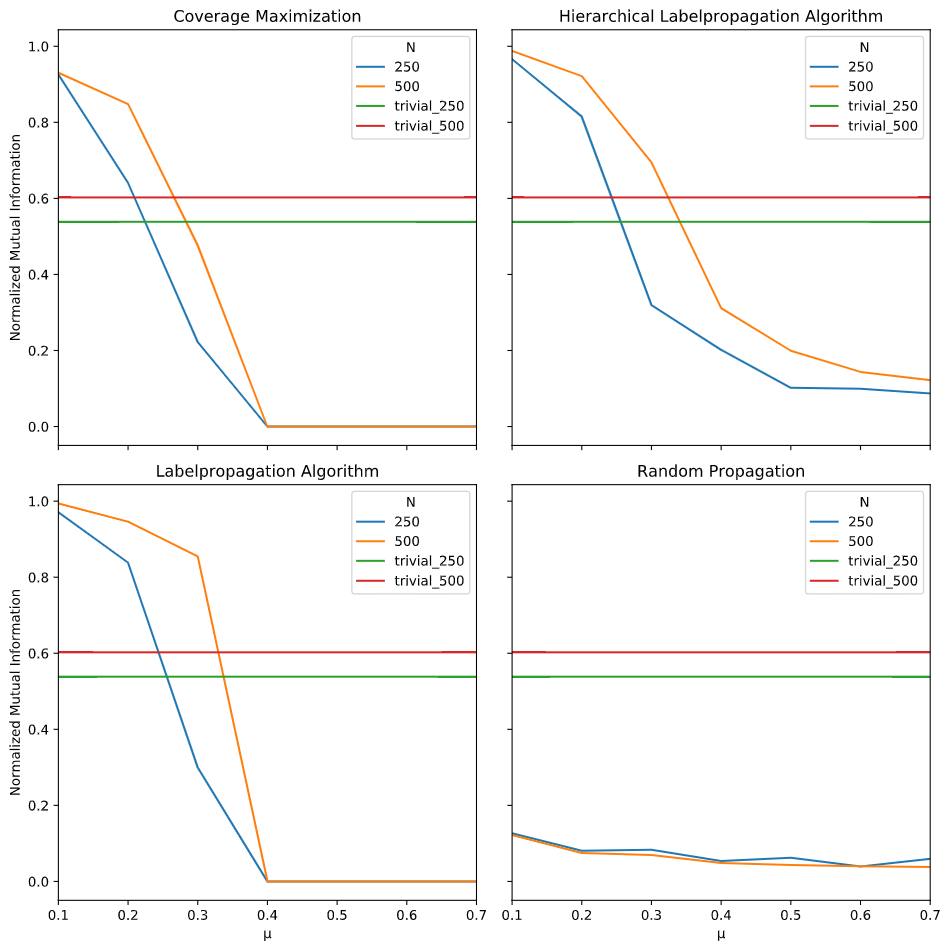
\includegraphics[width=\linewidth]{baselines.png}
  \caption{The figure shows the normalized mutual information performance results of the baseline models. The vertical lines refer to the trivial case of assigning each node an individual partition.}
  \label{fig:baseline}
\end{figure}

\subsection{Model results}
The Coverage Maximization model collapses similarly to the original label propagation after $\mu>0.3$. This was expected, as coverage fails to take characteristics of the graph into account. Meaning, that it only succeeds on graphs, whose main characteristic is their strong community structure. On the other hand, the Modularity model performs better than all of the other models. In Figure \autoref{fig:models} the MapEquation approach returns results for every $\mu$, but they remain below the Modularity approach. This shows that the MapEquation alone does not suffice to outperform modularity. Surprisingly, the node similarity method appears to be the second best model in this analysis. Although, not being as performant as the label propagation methods or coverage maximization for $\mu=0.1$, it quickly outperforms them as the mixing parameter increases. The first considerate drop in performance happens at $\mu=0.4$ which is interestingly also the declining point for label propagation and coverage maximization. The last observation which should be noted is that most models work better for larger graph sizes. However, this fact even holds for the trivial solution, hinting at issues with the general NMI comparison metric as it seems to favour larger graph sizes.

\begin{figure}[h]
  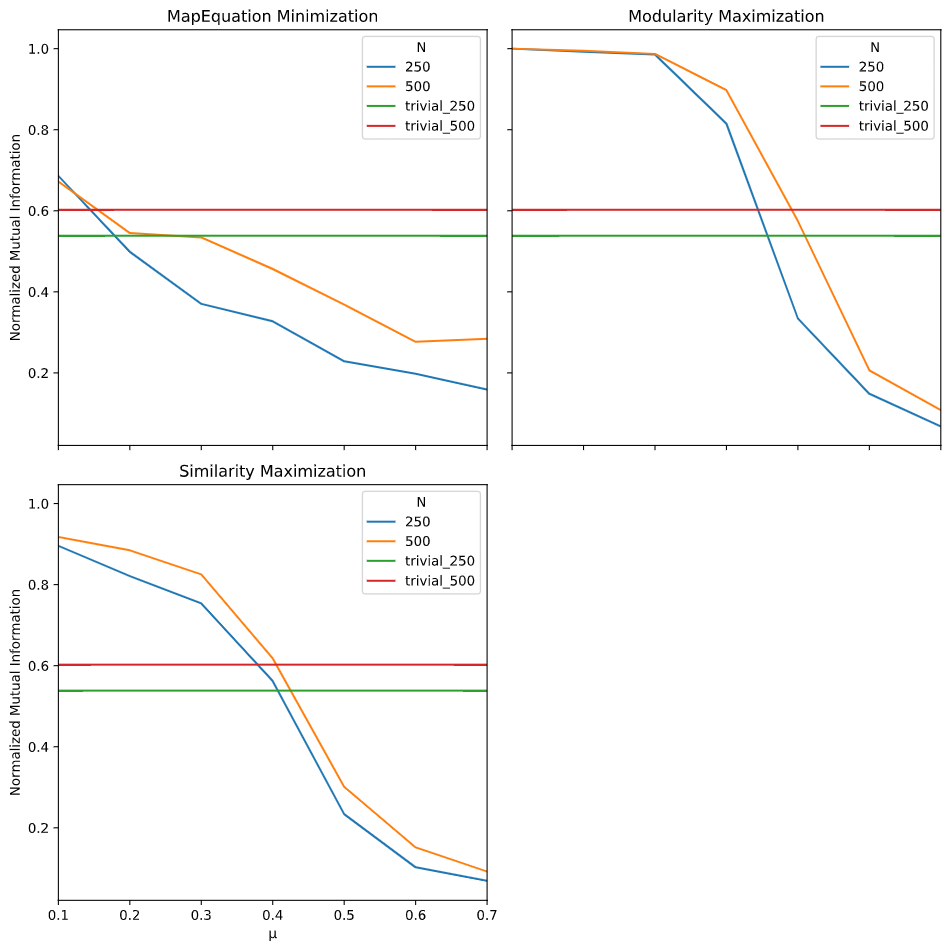
\includegraphics[width=\linewidth]{models.png}
  \caption{The figure shows the normalized mutual information performance results of each model. The vertical lines refer to the trivial case of assigning each node an individual partition.}
  \label{fig:models}
\end{figure}
% TODO: Thought that this only applies to certain quality functions
% TODO: The paper did not include time in the analysis as critis´cism. Also node cises were small 

\section{Discussion}
\label{sec:discussion}
This comparative analysis compared multiple models while keeping the algorithm fixed. With the results, the paper attempts to answer two important questions. First, how important is a sophisticated model for the community detection task? Second, which of the models is the most effective?
The results for Louvain largely reproduces the results from \citeauthor{lancichinetti_CommunityDetectionAlgorithms_2009}. With Louvain being among the top performing algorithms. However, according to this study the MapEquation based InfoMap outperformed the Louvain algorithm. This does not align with the results of this paper's MapEquation-based algorithm. The result is not suprising, as \citeauthor{bohlin_CommunityDetectionVisualization_2014} briefly mentions that further steps are required within the InfoMap algorithm, that can enable the reassignment of previously established communities and nodes. The Louvain-Core algorithm forcefully merges nodes into communities and that can lead to undesired outcomes later on. This hints at an intricate relationship between the algorithmic behaviour. The results clearly show the importance of sophisticated models for community detection tasks, but also their insufficiency to act as sole reason for their success. The Louvain algorithm for instance, performs much better than the \citeauthor{clauset_FindingCommunityStructure_2004} method, because it mitigates resolution short comings of Modularity. Leading to the conclusion, that the algorithm mainly serves to balance the shortcomings of a particular model. Henceforth, Louvain-Core is not a method which unanimously improves other models as its greedy aggregation behaviour proves to be too strong for some models. However, Louvain-Core seems to convert the global optimization attempt to one that is a more fine-grained local attempt, as seen in the Label Propagation case. 

As for the first question of this paper, it can be said that a more sophisticated model can indeed improve the behaviour of an algorithm for more complicated community structures. This is indicated in the sudden drop for both label propagation algorithms and the coverage maximization method, while more sophisticated models like Similarity, MapEquation and Modularity prevailed. However, it should be noted that "behaviour" refers to avoiding collapses and not general performance, as the best score for MapEquation could not reach the scores of simpler models like label propagation..  
The answer to the second question is clear. Louvain outperformed all the models evaluated in this comparative analysis. However, the node similarity model performed better than it popularity would suggest. 

However, there are still many directions to further this research. First, the graph sizes did not represent typical graphs as they are often larger. \citeauthor{lancichinetti_CommunityDetectionAlgorithms_2009} shows that the Louvain algorithm breaks down earlier for large network sizes. Also, this paper did not focus on time as performance criteria, even though it remains to be a crucial aspect of a method's effectiveness. The newly implemented node-similarity based model does appear to be fast as it mostly consists of fast matrix multiplications. The node-embeddings are quick to train on a GPU as well. However, the time should be investigated in a proper experimental setting. Furthermore, the model requires a multitude of hyperparameters and several decisions where made whose alternatives should have been investigated in greater detail. One example that was prelimarily investigated was the initialization of nodes, indicating that starting with every node in its partition indeed performs best. However, other decisions like word-vector reduction strategies or different distance functions where not looked into in detail.

\section{Summary}
\label{sec:summary}
To conclude, this paper not only showcased the influence of models for increasingly complex community structures but also their relationship to partitioning algorithms. Furthermore, this paper introduced two novel approaches. First, a louvain inspired hierarchical label propagation algorithm, which prevents the sudden collapse into one partition for higher mixing parameters. Second, a more sophistacted node-similarity based method leveraging the power of node-embeddings.

\newpage
\appendix
\section{The Similarity Maximization Algorithm}
This appendix further details some of the intricacies of the similarity maximization algorithm employed in this paper. Also some of the design decisions for reproduction purposes. As mentioned earlier, the method largely follows Louvain-Core. The difference applies to the initialization and the local movement phase. The initialization only applies once and trains the node-embeddings. While the local movement is shown in Algorithm \autoref{alg:glove}.
\begin{algorithm*}[htb]
\label{alg:glove}
\SetAlgoLined
\SetKwProg{Fn}{function}{ is}{end}
\SetKwInOut{Input}{input}
\Input{$P = \{C_1, C_2, ..., C_n\}$ \\ // P is a set of communities \\ $E \in \mathbb{R}^{n\times m}$ \\ // E is the embdedding matrix. \\ // n is the number of nodes and m the embedding size.}

\Fn{LocalMovement(Partition: init\_P, EmbeddingMatrix: E) : Partition}{
 \While{$\Delta Gain > Threshold$}{
    \If{$|P| <= 1$}{return $init\_P$;}\\
  Initialize random node sequence N;\\
  \ForEach{n in N}{
    Compute $\Delta ACD(n, C_n, E)$\\
    Select Community Candidates $I = C_{Adj(n)}\cup C_{new}$\\ 
    Find $C_{chosen}=\max_{i \in I}{\frac{\Delta ACD(i, C_i, E)* \Delta ACD(n, C_n, E)}{|C_i|}}$\\
    Update $C_n = C_{chosen}$ \\
    Compute $\Delta Gain = \frac{1}{|P|} \sum_{i \in I}{ACD(i, C_i, E)}$
  }
 }
}

\caption{Local movement with node-similarities}
\end{algorithm*}
The general algorithm is simple in essence. However, in order to function properly several implementation details are important. 

First, the algorithm ends either on breaking the threshold or if only one partition remains. In this case it is beneficial to reject the changes applied in the current iteration and just return the initial partition. Next, is the importance of \emph{Gain}. In the case the giving community gain is the difference between the modified community and the initial community. However, in the case of the receiving community it is the difference between the initial community and the modified community. Also, there are special cases that need to be considered while computing $\Delta ACD$. If a giving community is about to lose its last member or receiving community is about to receive its first member the difference is not zero as this renders the whole optimization function zero. It works better to specify a small constant for these cases. In this paper 0.00001 was used as the constant. This is especially important for the start of the algorithm as many communities will lose their last member. Other initialization schemes might account for this. An example would be to initialize the partitition by first assigning each node the partition of his closest neighbor. 

Second, The model used a set of hyperparameters to train the node embeddings. The random walk sequence went on for 100.000 steps. The embedding size was set to 30 and the context window was 2 in both directions (previous steps and future steps). It is not expected that the GloVe model parameters (embedding size and context window) have much influence on the performance. A particular focus on those is important for generalisation purposes. However, this model was allowed to overfit as a new set of node embeddings was trained with each new graph. Furthermore, these graphs did not change their structure over the course of the community detection process. This obviously, doesn't hold for evolving or changing graph settings. More important is the length random walk sequence. One long random walk was deemed as sufficient, as the markovian nature of the random walk makes the starting point of the random walk obsolete. Meaning, each step can be interpreted as starting point for an entirely new random walk. This makes sampling very efficient. However, this only applies to undirected graphs. In disconnected graphs or directed graphs the starting node holds crucial importance and co-occurrence sampling must be handled different. 

Third, a number of decision have been made to increase the performance of the model. The distance function was chosen to be the L2 difference as it show cased promising results. Other distance functions can also be considered, but it seemed as if the cosine-distance did not yield positive results. Next, for the node-embedding reduction the averaging method was chosen. However, one can also choose to retrain a new model for every iteration. This seems expensive, but the training of node-embeddings is in practise much faster as it would be for word embeddings. Meaning, for increasingly reduced graphs the training typically becomes cheaper. Same holds for the random walk to resample on the reduced graph. Another reduction approach would be to select the node-embedding which is closest to the actual centroid. This would mitigate for outlier influences. 


\section{Visualizing the effectiveness of Similarity Maximization}
This section includes some of the images that show the effectiveness of the algorithm.
Figure shows an example partition on a graph. It becomes clear that the model finds a sufficient partition. However, some partitions remain undetected. The issue seems related to resolution. The algorithm tends to be too detailed, whereas Modularity often tends to be too broad. One would expect the issue to be resolved on the next iteration by merging the super communities. However, this is not the case as the stopping criteria are too strong and lead to a subsequent collapse. In order to solve this issue, better stopping criteria must be reviewed which do not force the algorithm to collapse when the graph sizes are low in subsequent iterations of the Louvain-Core method.

\begin{figure}[h]
  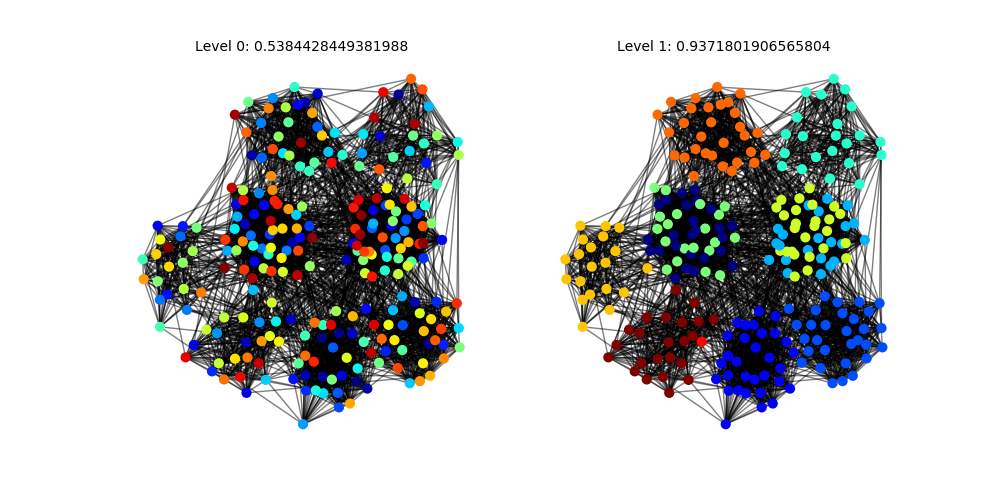
\includegraphics[width=\linewidth]{example.png}
  \caption{The figure shows the partitioning result of the similarity based method. The left side shows the trivial solution, while the subsequent graphs show different levels of the algorithm.}
  \label{fig:example}
\end{figure}

Figure \autoref{fig:detected} reinforces the previously established observation. The method is genrally strongly capable of detecting partitions. However, some partitions appear to be "split" into two separate partitions.

\begin{figure*}[h]
  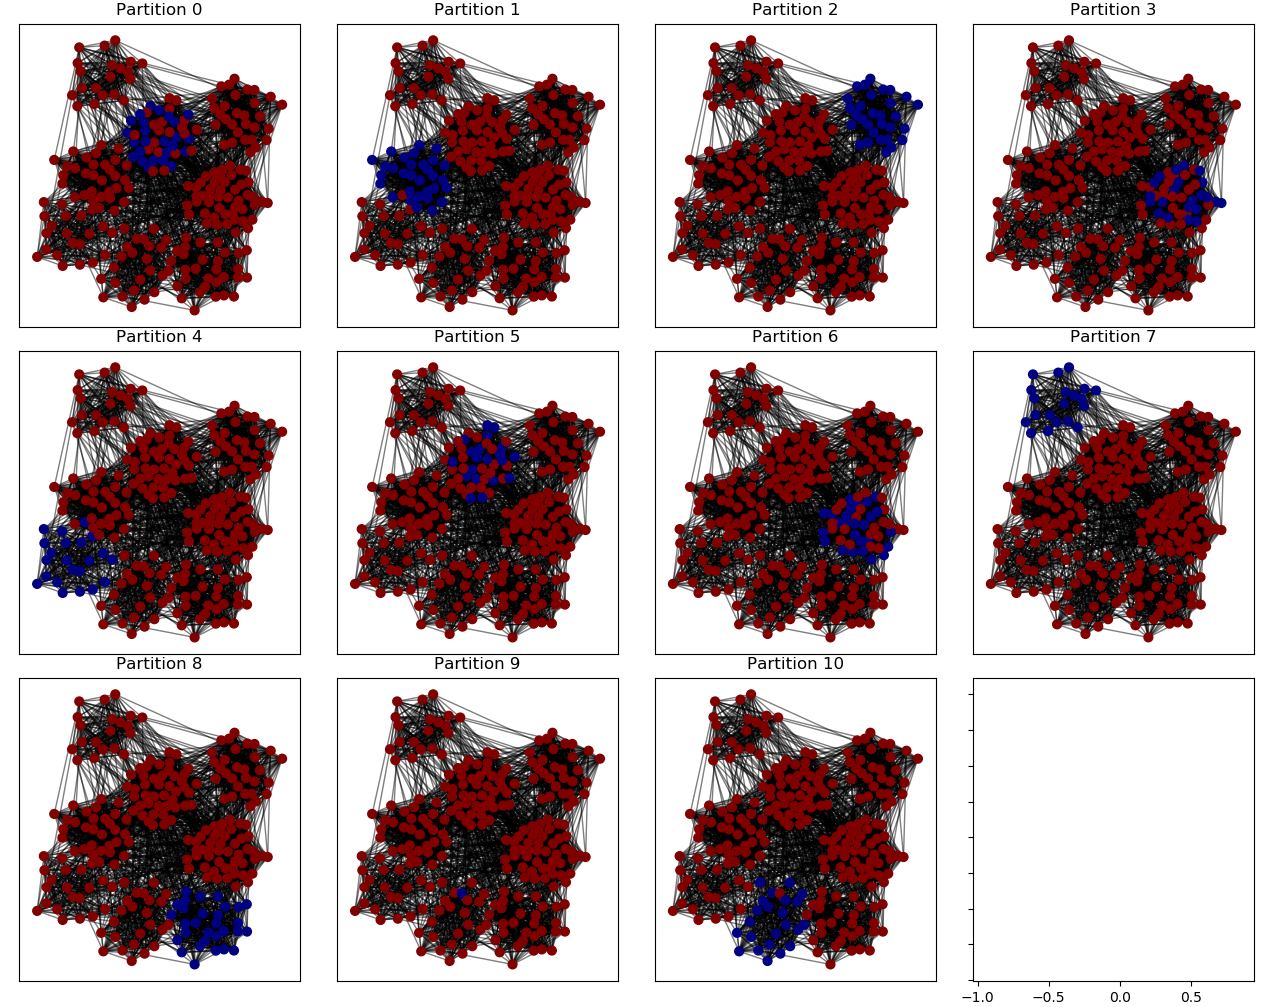
\includegraphics[width=\linewidth]{detected.png}
  \caption{The figure shows the partitions that have been identified by the algorithm. Each figure represents a community in blue.}
  \label{fig:detected}
\end{figure*}



\section{Code Repository}
The repository for this code is publicly available and can be downloaded on Github. It also provides additional information on how to execute the code. The repository can be found at \url{https://github.com/Olu93/project_network_science}

\newpage
\printbibliography
\end{document}
%%%%%%%%%%%%%%%%%%%%%%%%%%%%%%%%%%%%%%%%%%%%%%%%%%%%%%%%%%%%%%%%%%%%%%%%%%%%
\par
